\propriete[
    \exmplist
        {27,32 $\times$ 18,1 devient :\\ \opmul[shiftintermediarysymbol=\textcolor{gray}{0},displayshiftintermediary=all]{27.32}{18.1}}
        {8768$\times$12792 devient :\\ \opmul[shiftintermediarysymbol=\textcolor{gray}{0},displayshiftintermediary=all]{12792}{8768}}
        {0,0301$\times$11,2 devient :\\ \opmul[shiftintermediarysymbol=\textcolor{gray}{0},displayshiftintermediary=all]{11.2}{0.0301}}
    \rmq Si un nombre continent le chiffre 0, on peut directement sauter les multiplication par ce chiffre, puisqu'on sait qu'on obtiendra que des 0 (comme dans le troisième exemple).]
{Poser une multiplication}
{On va ici poser la multiplication 13,28 $\times$ 3,04.\\\vspace{1em}\\
\begin{minipage}{0.7\textwidth}    
On pose les deux nombres à additionner l'un en dessous de l'autre, celui avec le moins de chiffre en bas. On ignore les virgules, \textcolor{red}{on aligne donc les dernier chiffres}.  
\end{minipage}
\hfill
\begin{minipage}{0.22\textwidth}
    \begin{figure}[H]
    \centering
        \resizebox{\textwidth}{!}{
            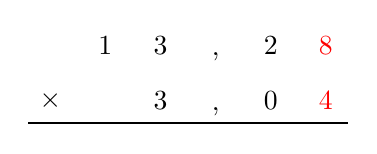
\begin{tikzpicture}[scale=0.7]
                \draw (0,0) node {1} ;
                \draw (1,0) node {3} ; 
                \draw (2,-0.2) node {,} ;
                \draw (3,0) node {2} ;
                \draw [red] (4,0) node {8} ;
                \draw (1,-1) node {3} ; 
                \draw (2,-1.2) node {,} ;
                \draw (3,-1) node {0} ;
                \draw [red] (4,-1) node {4} ;
                \draw (-1,-1) node {$\times$} ;
                \draw (-1.4,-1.4) -- (4.4,-1.4) ;
            \end{tikzpicture}
        }
    \end{figure}
\end{minipage}
\\\vspace{1em}\\
\begin{minipage}{0.7\textwidth}    
    On va multiplier tous les chiffres du nombre du haut par le dernier chiffre du nombre du bas, en commençant par la droite.
    On a donc \textcolor{red}{$4\times 8=32$}. On \textcolor{teal}{retient donc le 3} et on \textcolor{blue}{écrit le 2 en dessous}.
\end{minipage}
\hfill
\begin{minipage}{0.22\textwidth}
    \begin{figure}[H]
    \centering
        \resizebox{\textwidth}{!}{
            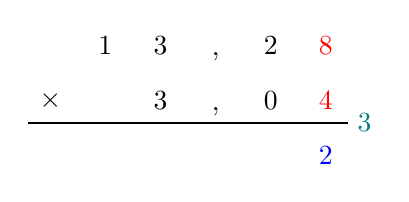
\begin{tikzpicture}[scale=0.7]
                \draw (0,0) node {1} ;
                \draw (1,0) node {3} ; 
                \draw (2,-0.2) node {,} ;
                \draw (3,0) node {2} ;
                \draw [red] (4,0) node {8} ;
                \draw (1,-1) node {3} ; 
                \draw (2,-1.2) node {,} ;
                \draw (3,-1) node {0} ;
                \draw [red] (4,-1) node {4} ;
                \draw [blue] (4,-2) node {2} ;
                \draw [teal] (4.7,-1.4) node {3} ;
                \draw (-1,-1) node {$\times$} ;
                \draw (-1.4,-1.4) -- (4.4,-1.4) ;
            \end{tikzpicture}
        }
    \end{figure}
\end{minipage}
\\\vspace{1em}\\
\begin{minipage}{0.7\textwidth}    
    On continue avec le chiffre suivant. \textcolor{red}{$4\times 2=8$}, mais on oublie pas notre retenue, 3. On a donc 8+3=11, \textcolor{blue}{on écrit donc 1} et \textcolor{teal}{on retient 1}. Comme on a utilisé le 3 qu'on avait retenue du calcul précédent, on peut le rayer pour ne pas s'embrouiller.
\end{minipage}
\hfill
\begin{minipage}{0.22\textwidth}
    \begin{figure}[H]
    \centering
        \resizebox{\textwidth}{!}{
            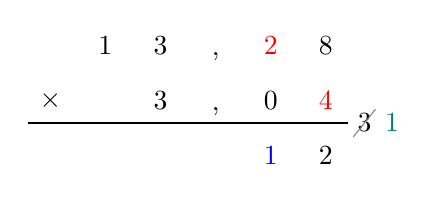
\begin{tikzpicture}[scale=0.7]
                \draw (0,0) node {1} ;
                \draw (1,0) node {3} ; 
                \draw (2,-0.2) node {,} ;
                \draw [red] (3,0) node {2} ;
                \draw (4,0) node {8} ;
                \draw (1,-1) node {3} ; 
                \draw (2,-1.2) node {,} ;
                \draw (3,-1) node {0} ;
                \draw [red] (4,-1) node {4} ;
                \draw (4,-2) node {2} ;
                \draw [blue] (3,-2) node {1} ;
                \draw (4.7,-1.4) node {3} ;
                \draw [gray] (4.5,-1.65) -- (4.9,-1.15) ;
                \draw [teal] (5.2,-1.4) node {1} ;
                \draw (-1,-1) node {$\times$} ;
                \draw (-1.4,-1.4) -- (4.4,-1.4) ;
            \end{tikzpicture}
        }
    \end{figure}
\end{minipage}
\\\vspace{1em}\\
\begin{minipage}{0.7\textwidth}    
    On continue jusqu'à avoir calculé avec tous les chiffres du nombre de haut. Avec la retenue, on a \textcolor{red}{$4\times 3=12$ et 12+1=13}, on retient donc 1, puis \textcolor{teal}{$4\times 1=4$ et 4+1=5}
\end{minipage}
\hfill
\begin{minipage}{0.22\textwidth}
    \begin{figure}[H]
    \centering
        \resizebox{\textwidth}{!}{
            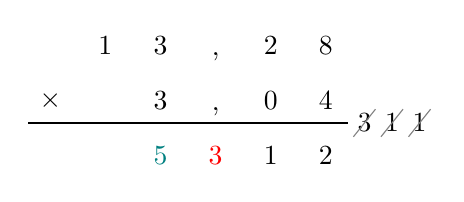
\begin{tikzpicture}[scale=0.7]
                \draw (0,0) node {1} ;
                \draw (1,0) node {3} ; 
                \draw (2,-0.2) node {,} ;
                \draw (3,0) node {2} ;
                \draw (4,0) node {8} ;
                \draw (1,-1) node {3} ; 
                \draw (2,-1.2) node {,} ;
                \draw (3,-1) node {0} ;
                \draw (4,-1) node {4} ;
                \draw (4,-2) node {2} ;
                \draw (3,-2) node {1} ;
                \draw [red] (2,-2) node {3} ;
                \draw [teal] (1,-2) node {5} ;
                \draw (4.7,-1.4) node {3} ;
                \draw [gray] (4.5,-1.65) -- (4.9,-1.15) ;
                \draw (5.2,-1.4) node {1} ;
                \draw [gray] (5,-1.65) -- (5.4,-1.15) ;
                \draw (5.7,-1.4) node {1} ;
                \draw [gray] (5.5,-1.65) -- (5.9,-1.15) ;
                \draw (-1,-1) node {$\times$} ;
                \draw (-1.4,-1.4) -- (4.4,-1.4) ;
            \end{tikzpicture}
        }
    \end{figure}
\end{minipage}
\\\vspace{1em}\\
\begin{minipage}{0.7\textwidth}    
    On passe ensuite à la ligne d'en dessous, qu'on commence par \textbf{un} \textcolor{red}{0} car on a déjà fait \textbf{un} chiffre.
\end{minipage}
\hfill
\begin{minipage}{0.22\textwidth}
    \begin{figure}[H]
    \centering
        \resizebox{\textwidth}{!}{
            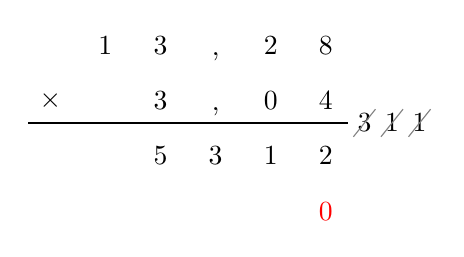
\begin{tikzpicture}[scale=0.7]
                \draw (0,0) node {1} ;
                \draw (1,0) node {3} ; 
                \draw (2,-0.2) node {,} ;
                \draw (3,0) node {2} ;
                \draw (4,0) node {8} ;
                \draw (1,-1) node {3} ; 
                \draw (2,-1.2) node {,} ;
                \draw (3,-1) node {0} ;
                \draw (4,-1) node {4} ;
                \draw (4,-2) node {2} ;
                \draw (3,-2) node {1} ;
                \draw (2,-2) node {3} ;
                \draw (1,-2) node {5} ;
                \draw [red] (4,-3) node {0} ;
                \draw (4.7,-1.4) node {3} ;
                \draw [gray] (4.5,-1.65) -- (4.9,-1.15) ;
                \draw (5.2,-1.4) node {1} ;
                \draw [gray] (5,-1.65) -- (5.4,-1.15) ;
                \draw (5.7,-1.4) node {1} ;
                \draw [gray] (5.5,-1.65) -- (5.9,-1.15) ;
                \draw (-1,-1) node {$\times$} ;
                \draw (-1.4,-1.4) -- (4.4,-1.4) ;
            \end{tikzpicture}
        }
    \end{figure}
\end{minipage}
\begin{minipage}{0.7\textwidth}    
    On passe recommence ensuite les multiplication, toujours de gauche à droite. \textcolor{red}{$0\times 8=0$}, \textcolor{blue}{$0\times 2=0$}, \textcolor{teal}{$0\times 3=0$} et \textcolor{violet}{$0\times 1=0$}
\end{minipage}
\hfill
\begin{minipage}{0.22\textwidth}
    \begin{figure}[H]
    \centering
        \resizebox{\textwidth}{!}{
            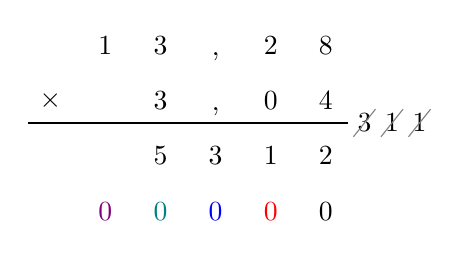
\begin{tikzpicture}[scale=0.7]
                \draw (0,0) node {1} ;
                \draw (1,0) node {3} ; 
                \draw (2,-0.2) node {,} ;
                \draw (3,0) node {2} ;
                \draw (4,0) node {8} ;
                \draw (1,-1) node {3} ; 
                \draw (2,-1.2) node {,} ;
                \draw (3,-1) node {0} ;
                \draw (4,-1) node {4} ;
                \draw (4,-2) node {2} ;
                \draw (3,-2) node {1} ;
                \draw (2,-2) node {3} ;
                \draw (1,-2) node {5} ;
                \draw (4,-3) node {0} ;
                \draw [red] (3,-3) node {0} ;
                \draw [blue] (2,-3) node {0} ;
                \draw [teal] (1,-3) node {0} ;
                \draw [violet] (0,-3) node {0} ;
                \draw (4.7,-1.4) node {3} ;
                \draw [gray] (4.5,-1.65) -- (4.9,-1.15) ;
                \draw (5.2,-1.4) node {1} ;
                \draw [gray] (5,-1.65) -- (5.4,-1.15) ;
                \draw (5.7,-1.4) node {1} ;
                \draw [gray] (5.5,-1.65) -- (5.9,-1.15) ;
                \draw (-1,-1) node {$\times$} ;
                \draw (-1.4,-1.4) -- (4.4,-1.4) ;
            \end{tikzpicture}
        }
    \end{figure}
\end{minipage}
\begin{minipage}{0.7\textwidth}    
    Même chose pour le dernier chiffre. Cette fois-ci, comme on a déjà fait 2 chiffre, \textcolor{olive}{la ligne commence avec 2 zéros}.\\
    Et on a  \textcolor{red}{$3\times 8=24$}, on retient 2. \textcolor{blue}{$3\times 2=6$, 8 avec la retenue }, \textcolor{teal}{$3\times 3=9$} et \textcolor{violet}{$3\times 1=3$}
\end{minipage}
\hfill
\begin{minipage}{0.22\textwidth}
    \begin{figure}[H]
    \centering
        \resizebox{\textwidth}{!}{
            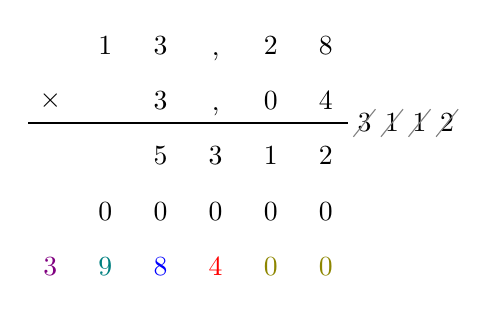
\begin{tikzpicture}[scale=0.7]
                \draw (0,0) node {1} ;
                \draw (1,0) node {3} ; 
                \draw (2,-0.2) node {,} ;
                \draw (3,0) node {2} ;
                \draw (4,0) node {8} ;
                \draw (1,-1) node {3} ; 
                \draw (2,-1.2) node {,} ;
                \draw (3,-1) node {0} ;
                \draw (4,-1) node {4} ;
                \draw (4,-2) node {2} ;
                \draw (3,-2) node {1} ;
                \draw (2,-2) node {3} ;
                \draw (1,-2) node {5} ;
                \draw (4,-3) node {0} ;
                \draw (3,-3) node {0} ;
                \draw (2,-3) node {0} ;
                \draw (1,-3) node {0} ;
                \draw (0,-3) node {0} ;
                \draw [olive] (4,-4) node {0} ;
                \draw [olive] (3,-4) node {0} ;
                \draw [red] (2,-4) node {4} ;
                \draw [blue] (1,-4) node {8} ;
                \draw [teal] (0,-4) node {9} ;
                \draw [violet] (-1,-4) node {3} ;
                \draw (4.7,-1.4) node {3} ;
                \draw [gray] (4.5,-1.65) -- (4.9,-1.15) ;
                \draw (5.2,-1.4) node {1} ;
                \draw [gray] (5,-1.65) -- (5.4,-1.15) ;
                \draw (5.7,-1.4) node {1} ;
                \draw [gray] (5.5,-1.65) -- (5.9,-1.15) ;
                \draw (6.2,-1.4) node {2} ;
                \draw [gray] (6,-1.65) -- (6.4,-1.15) ;
                \draw (-1,-1) node {$\times$} ;
                \draw (-1.4,-1.4) -- (4.4,-1.4) ;
            \end{tikzpicture}
        }
    \end{figure}
\end{minipage}
\begin{minipage}{0.7\textwidth}    
    Il ne reste plus qu'à additionner colone par colone les résultats obtenus, comme une addition posée.\\
    Et on a  \textcolor{red}{$2+0+0=2$}. \textcolor{blue}{$1+0+0=1$}, \textcolor{teal}{$3+0+4=7$}, \textcolor{violet}{$5+0+8=3$}, on retient 1. \textcolor{olive}{1+0+9=10}, on retient 1 et \textcolor{orange}{1+3=4}.
\end{minipage}
\hfill
\begin{minipage}{0.22\textwidth}
    \begin{figure}[H]
    \centering
        \resizebox{\textwidth}{!}{
            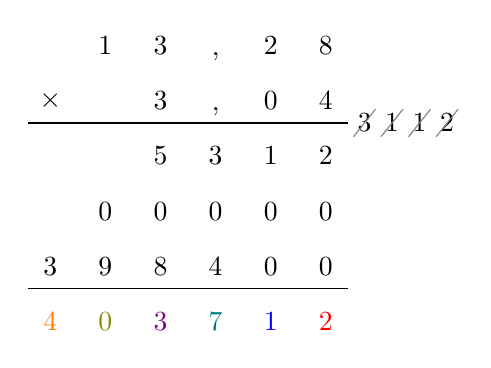
\begin{tikzpicture}[scale=0.7]
                \draw (0,0) node {1} ;
                \draw (1,0) node {3} ; 
                \draw (2,-0.2) node {,} ;
                \draw (3,0) node {2} ;
                \draw (4,0) node {8} ;
                \draw (1,-1) node {3} ; 
                \draw (2,-1.2) node {,} ;
                \draw (3,-1) node {0} ;
                \draw (4,-1) node {4} ;
                \draw (4,-2) node {2} ;
                \draw (3,-2) node {1} ;
                \draw (2,-2) node {3} ;
                \draw (1,-2) node {5} ;
                \draw (4,-3) node {0} ;
                \draw (3,-3) node {0} ;
                \draw (2,-3) node {0} ;
                \draw (1,-3) node {0} ;
                \draw (0,-3) node {0} ;
                \draw (4,-4) node {0} ;
                \draw (3,-4) node {0} ;
                \draw (2,-4) node {4} ;
                \draw (1,-4) node {8} ;
                \draw (0,-4) node {9} ;
                \draw (-1,-4) node {3} ;
                \draw [red] (4,-5) node {2} ;
                \draw [blue] (3,-5) node {1} ;
                \draw [teal] (2,-5) node {7} ;
                \draw [violet] (1,-5) node {3} ;
                \draw [olive] (0,-5) node {0} ;
                \draw [orange] (-1,-5) node {4} ;
                \draw (4.7,-1.4) node {3} ;
                \draw [gray] (4.5,-1.65) -- (4.9,-1.15) ;
                \draw (5.2,-1.4) node {1} ;
                \draw [gray] (5,-1.65) -- (5.4,-1.15) ;
                \draw (5.7,-1.4) node {1} ;
                \draw [gray] (5.5,-1.65) -- (5.9,-1.15) ;
                \draw (6.2,-1.4) node {2} ;
                \draw [gray] (6,-1.65) -- (6.4,-1.15) ;
                \draw (-1,-1) node {$\times$} ;
                \draw (-1.4,-1.4) -- (4.4,-1.4) ;
                \draw (-1.4,-4.4) -- (4.4,-4.4) ;
            \end{tikzpicture}
        }
    \end{figure}
\end{minipage}
\begin{minipage}{0.7\textwidth}    
    Enfin, on place la virgule. On compte le nombre de chiffre derrière la virgule pour nos nombres de départ. 13,\textbf{28} a deux chiffres derrière la virgule. Pareil pour 3,\textbf{04}, ce qui nous fait un total de 4 chiffres derrière la virgule. 
    \\Le résultat final aura donc 4 chiffres derrière la virgule.
\end{minipage}
\hfill
\begin{minipage}{0.22\textwidth}
    \begin{figure}[H]
    \centering
        \resizebox{\textwidth}{!}{
            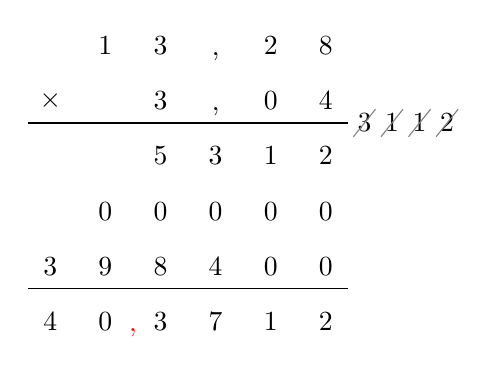
\begin{tikzpicture}[scale=0.7]
                \draw (0,0) node {1} ;
                \draw (1,0) node {3} ; 
                \draw (2,-0.2) node {,} ;
                \draw [red] (0.5,-5.2) node {,} ;
                \draw (3,0) node {2} ;
                \draw (4,0) node {8} ;
                \draw (1,-1) node {3} ; 
                \draw (2,-1.2) node {,} ;
                \draw (3,-1) node {0} ;
                \draw (4,-1) node {4} ;
                \draw (4,-2) node {2} ;
                \draw (3,-2) node {1} ;
                \draw (2,-2) node {3} ;
                \draw (1,-2) node {5} ;
                \draw (4,-3) node {0} ;
                \draw (3,-3) node {0} ;
                \draw (2,-3) node {0} ;
                \draw (1,-3) node {0} ;
                \draw (0,-3) node {0} ;
                \draw (4,-4) node {0} ;
                \draw (3,-4) node {0} ;
                \draw (2,-4) node {4} ;
                \draw (1,-4) node {8} ;
                \draw (0,-4) node {9} ;
                \draw (-1,-4) node {3} ;
                \draw (4,-5) node {2} ;
                \draw (3,-5) node {1} ;
                \draw (2,-5) node {7} ;
                \draw (1,-5) node {3} ;
                \draw (0,-5) node {0} ;
                \draw (-1,-5) node {4} ;
                \draw (4.7,-1.4) node {3} ;
                \draw [gray] (4.5,-1.65) -- (4.9,-1.15) ;
                \draw (5.2,-1.4) node {1} ;
                \draw [gray] (5,-1.65) -- (5.4,-1.15) ;
                \draw (5.7,-1.4) node {1} ;
                \draw [gray] (5.5,-1.65) -- (5.9,-1.15) ;
                \draw (6.2,-1.4) node {2} ;
                \draw [gray] (6,-1.65) -- (6.4,-1.15) ;
                \draw (-1,-1) node {$\times$} ;
                \draw (-1.4,-1.4) -- (4.4,-1.4) ;
                \draw (-1.4,-4.4) -- (4.4,-4.4) ;
            \end{tikzpicture}
        }
    \end{figure}
\end{minipage}
\\\vspace{1em}\\
Ainsi, on a trouvé 28 $\times$ 3,04=40,3712.
}
